\documentclass[10pt]{article}
\usepackage[utf8]{inputenc}
\usepackage{array, xcolor, bibentry}
\usepackage[margin=3cm]{geometry}

\usepackage[english]{babel}
\selectlanguage{english}

\usepackage{graphicx}
\graphicspath{ {./img/} }

\title{\bfseries M. Joaquín García González}
\author{manliojoaquin@gmail.com}
\date{}

\definecolor{lightgray}{gray}{0.8}
\newcolumntype{L}{>{\raggedleft}p{0.18\textwidth}}
\newcolumntype{R}{p{0.8\textwidth}}
\newcommand\VRule{\color{lightgray}\vrule width 0.5pt}

\begin{document}
    \pagenumbering{gobble}% Remove page numbers (and reset to 1)

    \maketitle

    \begin{minipage}[ht]{0.48\textwidth}
        Urb. Porlier, Módulo ``o'', Nº 8\\
        C/ General, Bajamar 38250\\
        San Cristóbal de La Laguna\\
        \\
        Nationality: Spanish, Argentinian\\
        Birth date: October 29th, 1990\\
        Telephone: +34 655 141 227
    \end{minipage}
    \begin{minipage}[ht]{0.48\textwidth}
        \begin{flushright}
        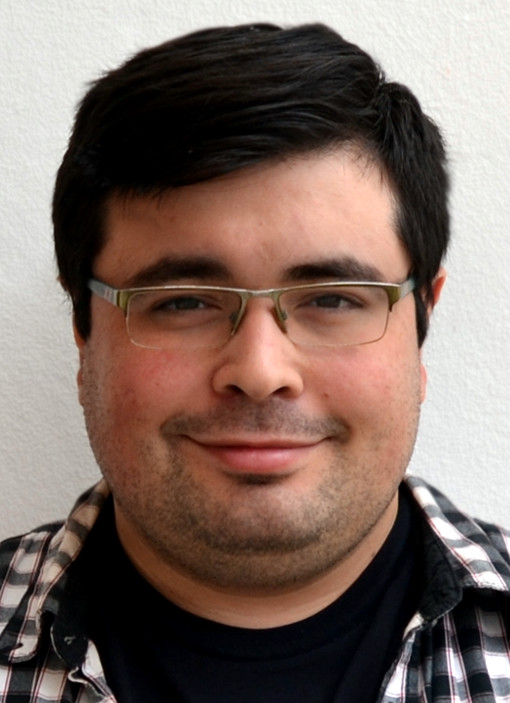
\includegraphics[height=8em]{profile}
        \end{flushright}
    \end{minipage}

    \section*{Usual tasks}
    \begin{itemize}
        \item Administration of computer equipment based on GNU-Linux and Windows.

        \item Development of web pages, mobile applications and standard software.

        \item Assembly and repair of desktop PCs, laptops and network infrastructure.

        \item Design of graphic materials, interfaces and products.
    \end{itemize}

    \section*{Programming languages}
    \begin{center}
    \begin{tabular}{ c c c c c c c c c c }

        Ruby & C\# & PHP & Bash & CSS & HTML & Javascript & \LaTeX & Unity-Script & Elixir

    \end{tabular}
    \end{center}

    \section*{Languages}
    \begin{tabular}{L!{\VRule}R}

        Spanish&Mother tongue\\\\

        English&Fluent (B2 certificate by the official language school of La Laguna in 2009.)\\\\

    \end{tabular}

    \section*{Personal Interests}
    Technology has always been present in my home, and together with games and music are the core of my interests. I first learned the basics of programming while building adventure modules for “Neverwinter Nights”. Nowadays my wife and I still run game sessions at home, which looks like half music store and half game workshop. I also play music in a band with students and former students of the computer science faculty and practice martial arts.

    \section*{Professional Experience}
    \begin{tabular}{L!{\VRule}R}
        2016--Now&{{\bf Freelance Full Stack Developer.}\newline I have been developing webs and specialized tools for private clients using a stack inspired in Jekyll simplicity, with MongoDB as a database engine, Ruby for the REST API and AngularJS for the front end, and using Angular-Material or Zurb-Foundation depending on the needs of each project.}\\\\

        2015--2016&{{\bf Administration of a computer room under the management of the Office of Free Software for the University of La Laguna.}\newline The University of La Laguna has it's own Linux distro based on Ubuntu, and all computer rooms has it installed. I was fortunate enough to get a job doing maintenance in the central computer room under the supervision of the Free Software Office of the university. There I learned a lot about automating tasks and diagnose hardware and software problems.}\\\\

        2015--2016&{{\bf Technical service for the company Horizont Atlantic SL.}\newline While working at the university, I wanted to get some experience in a non-academy environment. I got in touch with a close business, where they needed help and advice with technology related tasks, but didn't want to hire an engineer full time. Although I could not convince them to switch most of their operations to the cloud, I did convince them to get a raid, schedule backups and do a few more improvements. They even made the switch to linux and were able to work from home using sshfs under the hood.}\\\\

        2011--2014&{{\bf Development of video games for the company 4D3 Studio.}\newline I got the chance to work in a small studio developing in Unity3D, and at the same time learning from programmers, game designers and digital artists with first hand experience on the field, but the most important lessons from this period were about the interaction with clients, managers and other team members in a structured environment. }\\\\

        2014&{{\bf Design of geolocated mobile video game ``Progrezz''}\newline I got in contact with the Progrezz team while learning about geolocated experiences. I worked mainly in the game design and mechanics, and earned a lot of experience writing documentation for small teams.}\\\\

        2014&{{\bf Collaborating member in the organization and layout of the ``XV International Congress of Human Computer Interaction 2014'', held in
        Puerto de la Cruz in September 2014}\newline My tasks were mainly related with the making of the event's minutes. Most of them were a mix of different formats, and I had to build a coherent document from them, but I learned a lot about scripting and documentation research.}\\\\

        2011--2012&{{\bf Collaboration in the development of the Mundo Isla video game for the University of La Laguna in the project for the promotion of healthy habits ``SAVEH''}\newline I began in this project as a game designer, but the need of extra help with technical tasks helped me make the transition of programming as a hobby to programming as a job. During this time I re-learned the basics, specially about patterns and anti-patterns.}\\\\

        2009--2012&{{\bf Billboards for degrees of the University of La Laguna.}\newline La Laguna University held degrees about game design and 3D modeling. I got the chance to design the billboards for these degrees, and in doing so meet many members of the faculty who were also professionals of the field and learned the basics of game design and programming in the industry.}\\\\

    \end{tabular}

    \section*{Volunteering and Free Software}
    \begin{tabular}{L!{\VRule}R}

        2009&{Technical volunteer at the free software event ``Gran Canaria Desktop Summit''}\\\\

    \end{tabular}

    \section*{Imparted courses}
    \begin{tabular}{L!{\VRule}R}

        2014&{Speaker at the First Summer Scientific Campus in the Innovation Area of the General Foundation of the University of La Laguna.}\\\\

        2013--2014&{Computer classes at user level to individuals.}\\\\

        2013&{Teacher of the workshop ``Introduction to HTML5 and CSS3'' for the General Foundation of the University of La Laguna.}\\\\

        2013&{Teacher of the workshop ``Videogames Level 1: Project'' for the General Foundation of the University of La Laguna.}\\\\

        2012--2013&{Teacher of robotics at Nuriana S.L. (La Laguna).}\\\\

    \end{tabular}

    \section*{Academic training}
    \begin{tabular}{L!{\VRule}R}

        Now&{\bf Currently studying: }Upper grade training cycle in the development of multiplatform applications.\\\\

        2010&Bachelor's degree with specialization in Humanities and Social Sciences. CEAD Santa Cruz de Tenerife Mercedes Pinto.\\\\

        2007--2008&Cultural exchange to Australia. Certified by AFS Intercultura.\\\\[5pt]

    \end{tabular}

    \section*{Professional training}
    \begin{tabular}{L!{\VRule}R}

        2014&Training in web programming languages and systems administration, 240 Theoretical-practical hours. Certified by Fotón Sistemas Inteligentes. September 2014.\\\\

        2011&Introduction workshop to Adobe Flash, 20 Theoretical-practical hours. Certified by the Business Foundation of the University of La Laguna. May 2011.\\\\

        2009--2010&III Course of traditional animation and cartoons, 830 Theoretical-practical hours. Certified by La Mirada Producciones. July 2010.\\\\

    \end{tabular}

    \section*{Other merits}
    \begin{tabular}{L!{\VRule}R}

        &Coauthor of the article ``Promoting and Supporting Healthy Living By Design'' in the minutes of the INTERACT 2011 conference.\\\\

    \end{tabular}

    \section*{Known Software}
    \begin{tabular}{L!{\VRule}R}

        Development environments&Vim, Brackets, Unity3D, Atom.\\\\

        Version control&Git.\\\\

        Collaborative tools&Telegram, Slack, Trello, IRC, Git-Hub.\\\\

        Operative systems&GNU-Linux, Android and Windows (usual administrator), OSX (occasional administrator).\\\\

        Computer aided design and image manipulation&Imagemagick, Adobe Photoshop, Adobe Ilustrator, 3D Studio, Gimp, Inkscape and others.\\\\

    \end{tabular}


    \bibliographystyle{plain}
    \nobibliography{publication}

    {\bf\scriptsize\vfill\hfill In La Laguna, \today.}
\end{document}
